\section{Introduction}\label{sec:introduction}

A \emph{domain} is a nonempty connected open set. A \emph{circle domain}
in the Riemann sphere $\Chat$ is a domain whose complementary components
are closed round disks or single points. Koebe's
\emph{Kreisnormierungsproblem}, posed in 1908 \cite{Koebe1908}, asks
whether every planar domain has such a conformal model.

\begin{theorem}[Circle-domain uniformization]\label{thm:main}
Every nonempty connected open set $G\subset\Chat$ is conformally equivalent
to a circle domain.
\end{theorem}

This proves Koebe's conjecture in its unrestricted form.  The difficulty
is to control all complementary components at once.
There may be uncountably many of them, with no regularity or separation.
Even when finitely connected approximations have round complementary
disks, a limiting complementary component can contain more than the
disk obtained by following one of those disks to the limit. The proof
must rule out that excess and also control components for which no disk
has been followed.

Our construction chooses a countable set of complementary components
to mark. Write $b$ for the label of a source component. For a limiting
conformal map $f$, write $K_b(f)$ for the corresponding complementary
component of $f(G)$. At a marked
component, the finite approximations supply a distinguished round disk
$D_b\subset K_b(f)$, possibly reduced to a point. We arrange that
\[
 \begin{cases}
 K_b(f)\text{ is a singleton},& b\text{ unmarked},\\
 K_b(f)=D_b,& b\text{ marked}.
 \end{cases}
\]
These are the two geometric conclusions needed for the theorem.
Figure~\ref{fig:protrusion} illustrates the second obstruction. The
component correspondence and the inclusion $D_b\subset K_b(f)$ are
proved in Section~\ref{sec:transfer}.

\begin{figure}[tb]
\centering
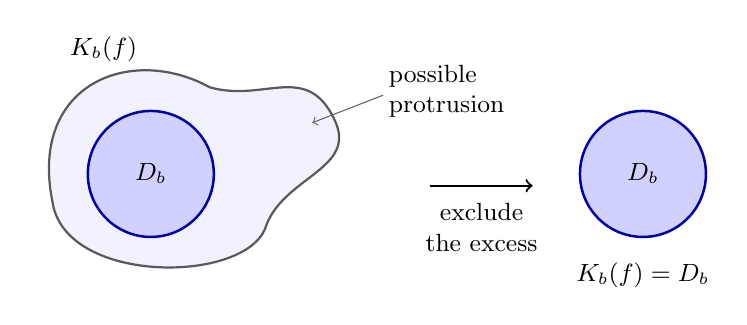
\begin{tikzpicture}[x=1cm,y=1cm,font=\small]
 \filldraw[fill=blue!5,draw=black!65,line width=.8pt]
 (-1.6,-.2) .. controls (-1.9,1.3) and (-.6,1.8) .. (.4,1.25)
 .. controls (1.1,1.05) and (1.65,1.6) .. (2,.8)
 .. controls (2.25,.2) and (1.3,.1) .. (1.1,-.55)
 .. controls (.8,-1.25) and (-1.45,-1.25) .. (-1.6,-.2);
 \filldraw[fill=blue!18,draw=blue!65!black,line width=.9pt]
 (-.35,.15) circle (.8);
 \node at (-.35,.15) {$D_b$};
 \node[above] at (-.95,1.45) {$K_b(f)$};
 \draw[->,black!60] (2.6,1.15)--(1.7,.8);
 \node[right,align=left] at (2.55,1.2) {possible\\protrusion};
 \draw[->,line width=.8pt] (3.2,0)--(4.5,0);
 \node[below,align=center] at (3.85,-.1) {exclude\\the excess};
 \filldraw[fill=blue!18,draw=blue!65!black,line width=.9pt]
 (5.9,.15) circle (.8);
 \node at (5.9,.15) {$D_b$};
 \node[below] at (5.9,-.85) {$K_b(f)=D_b$};
\end{tikzpicture}
\caption{A distinguished disk may initially be only part of a limiting
complementary component. The marked-component argument excludes every
such protrusion. This is a schematic picture; no boundary regularity of
$K_b(f)$ is assumed.}
\label{fig:protrusion}
\end{figure}


\subsection{From finite uniformization to boundary control}

Koebe proved the finite-connectivity theorem; see his 1920 treatment
\cite{Koebe1920}. He and Schramm established the countably connected
case \cite[Theorem~0.1]{HeSchramm1993}. Schramm introduced transboundary
extremal length and gave another proof, as well as uniformization results
for domains bounded by points and $K$-quasicircles for a fixed $K$
\cite{Schramm1995}.  These results combine
finite conformal approximation with estimates controlling which
boundary components survive the limit.

Geometric conditions also yield circle-domain models beyond countable
connectivity.  Esmayli and Rajala proved uniformization for cospread
domains, and more generally under a uniform quasitripod condition and
a packing bound \cite[Theorem~1.3 and Corollary~1.6]{EsmayliRajala2026}.
Karafyllia and Ntalampekos established the conjecture for spherical
Gromov-hyperbolic domains, obtaining uniform circle-domain models and
M\"obius uniqueness \cite[Theorem~1.2]{KarafylliaNtalampekos2024}.
Theorem~\ref{thm:main} imposes no geometric condition on the complement.

Finite approximations alone do not settle the limiting problem.
Rajala showed that arbitrary interior exhaustions can fail to have
circle-domain limits, and proved an exhaustion refinement theorem for
countably connected domains \cite[Theorems~1.1--1.3]{Rajala2025}.
Combining Theorem~\ref{thm:main} with Ntalampekos and Rajala's
exhaustion theorem \cite[Theorem~1.1]{NtalampekosRajala2025} gives an
unconditional fixed-domain approximation: every proper domain
$G\subsetneq\Chat$ has an exhaustion $G_j\subset G_{j+1}$,
$\bigcup_jG_j=G$, by finitely connected domains bounded by finitely many
disjoint Jordan curves lying in $G$. Fix three distinct points
$a_1,a_2,a_3\in G_1$. The conformal uniformizations
$f_j:G_j\to D_j$ onto finitely connected circle domains, normalized by
$f_j(a_k)=a_k$ for $k=1,2,3$, converge locally uniformly in the spherical
metric along the whole sequence to a conformal homeomorphism of $G$
onto a circle domain. For $G=\Chat$, the identity gives the trivial case.
This asserts the existence of a suitable exhaustion, not convergence
for arbitrary exhaustions. For further history, see \cite{Ntalampekos2026}.

We obtain the required control by choosing analytic tests on $G$ before
taking finite uniformizations.  A crucial freedom is to retain the
original conformal structure on each compact core while choosing a new
structure on its finite completion.  The core eventually exhausts the
whole domain, so the limiting map is conformal in the original
structure.  The tests are real functions or functions
with additive period one around a selected component. Each has finite
Dirichlet energy and a square-summable bound on its oscillation at the
complementary components. Small real barriers collapse unmarked
components; period-one tests detect a protrusion beyond a marked disk
through a boundary integral.

The mixed use of domain energy and boundary weights belongs to the
transboundary extremal-length approach introduced by Schramm
\cite{Schramm1995}.  Our path construction charges repeated boundary
visits individually and records portions traveling in earlier level
sets.  The law duality is a form of Fuglede's modulus for measure
systems \cite{Fuglede1957}, with the probability-measure duality
of Ambrosio, Di Marino, and Savar\'e
\cite{AmbrosioDiMarinoSavare2015}.  The additional tasks here are
to fuse the countable tests into one law controlling all boundary components,
to preserve compatibility as tests are appended, and to exclude all
possible noncircular limiting components.

\subsection{Proof overview}

Collapse each complementary component of $G$ to one point. The quotient
$X$ is a topological sphere, and $B=X\setminus G$ is compact and totally
disconnected. Thus $B$ supplies the labels $b$ used above. We use the
topology of $X$ to approach components, while retaining the original
conformal structure on $G$ for length and energy.

Section~\ref{sec:setup} defines the tests and their compatibility
condition. Compatibility controls how the level sets of a new test
meet continua formed from earlier levels. It permits the simultaneous
transfer in Section~\ref{sec:transfer}: finitely many tests extend to a
finite conformal completion, agree with the originals on a prescribed
compact core, and acquire arbitrarily little additional energy or
excess boundary oscillation. Their periods are preserved exactly. The
conformal structure may change outside the core; the cores eventually
exhaust $G$. Finite circle-domain uniformization then produces the
limits and component correspondence described above.

The tests themselves come from a boundary alternative. Either an end
can be separated from a fixed interior anchor by a small compatible
barrier, or there is a probability law of paths from the anchor to that
end with controlled mean arclength occupation. Section~\ref{sec:barriers}
constructs the barriers using paths that may run through complementary
components. Tags record portions lying in previously chosen level sets;
the remaining boundary contacts obey explicit incidence bounds. These
conditions allow paths to be spliced near their ends without losing the
estimates.

Section~\ref{sec:laws} proves the alternative. We use the
modulus--probability duality of Ambrosio, Di Marino, and Savar\'e
\cite{AmbrosioDiMarinoSavare2015}, proving the required measure-family
form in full. This first gives a path law for each prescribed countable
set of boundary tests and each atomless test measure. A separate fusion
argument produces \emph{one} law whose hit probabilities have bounded
counting $\ell^2(B)$ norm on the entire, possibly uncountable, set $B$.
Expected visit counts on previously prescribed countable sets are
controlled separately.

Section~\ref{sec:selection} removes diffuse intersections between
independent path laws. A four-path crossing argument then shows that
only countably many ends can lack small barriers. Selecting countably
many barriers gives a countable marked set $S\subset B$ and collapses
every $K_b(f)$ with $b\notin S$. This conclusion survives every later
countable compatible extension of the tests.

Section~\ref{sec:streams} handles the marked components. Averaging the
integer indices of lifted simple arcs produces period-one tests with
small energy and small oscillation away from the selected end. A
Stokes estimate turns these bounds into an upper bound on a boundary
integral. A protrusion would force a strictly larger lower bound.
Each such test excludes a neighborhood of a possible pair $(f,D_b)$;
second countability permits a countable selection excluding all pairs
with $D_b\ne K_b(f)$. The final simultaneous transfer proves
Theorem~\ref{thm:main}.

Theorem~\ref{thm:retained-tests} records the same construction with
an arbitrary prescribed countable compatible list retained from the outset.
For a finite family of bounded continuous real functions on $X$,
smooth with finite
Dirichlet energy on $G$, the simple sufficient condition
$\area((u_i,u_j)(B))=0$ for distinct tests gives exact agreement on
exhausting cores, vanishing tail energy, and vanishing square-summed
boundary oscillations; see Corollary~\ref{cor:scalar-retained-tests}.
This quantitative conclusion supplies the analytic input for the
removable-boundary rigidity companion \cite{OpenAIRigidity2026}.

Section~\ref{sec:hyperbolic} derives the geometric consequence from
Luo and Wu's Theorem~1.1(a) \cite{LuoWu2024}: every complete hyperbolic
surface of genus zero is intrinsically realized by the boundary of a
hyperbolic convex hull whose ideal set has round-disk or point components.

\subsection{Conventions and classical inputs}

The classical inputs are finite circle-domain uniformization, compact
genus-zero uniformization, Moore's decomposition theorem, area and
coarea, and standard Borel selection and refinement theorems. They are
cited where used. All constructions of compatible tests, fusion of
laws, and component exclusions are proved below.

Path laws are Borel probability measures on the stated code spaces.
We use their completions for universally measurable selections and
analytic events, and take the resulting laws on the Borel
sigma-algebra. Every nonnegative sum over an arbitrary index set is the
supremum of its finite subsums. In particular, every $\ell^2$ function
has countable positive support.
